\chapter{parreset}

\section{Introduction}

An LPE may have parameters of which the values are not used anymore after a particular state.
If such parameters can have different values after that state, they continue to add states to the state space for each of those values -- \emph{without} adding any new behavior!

The \texttt{parreset} command tries to determine whether the value of a parameter is used by an LPE after a particular summand.
If this is the case, the parameter is said to be \emph{relevant} for that summand; otherwise, the summand can `reset' the parameter, meaning that it can be assigned a default value.

To determine the relevance of parameters, \texttt{parreset} analyzes the reachability of summands in a generalized, symbolic manner.
The \texttt{datareset} command, serving a similar purpose (see \ref{datareset}), does a control-flow analysis instead.

\section{Formal background}

\subsection{Possible successors} \label{possiblesuccessors}

Consider summands $s_\alpha$ and $s_\beta$, referencing their elements conform \ref{summandelements}.
Summand $s_\beta$ is said to be a \emph{possible successor} of $s_\alpha$ if the following expression \emph{could be} satisfiable:
\begin{align*}
g_\alpha \land {g_\beta}[v \rightarrow q(v) \;|\; v \in \varsof{g_\beta} \setminus P][p \rightarrow v_\alpha(p) \;|\; p \in P]
\end{align*}

where $q(v)$ is a bijective function that relates variable $v$ to a fresh variable.

\section{Algorithm}

The algorithm is a generalization of an existing algorithm \cite{van2009state}.
It consists of two phases.

During the first phase (the preparation phase), we determine all successors of each summand of the LPE using the equation from the previous section.

The second phase (the iteration phase) follows these steps:

\begin{enumerate}

\item For each summand $s_\alpha$ of the LPE, create a set $R_\alpha$ that contains all parameters of the LPE.
This means that, initially, we assume that all parameters of the LPE are used by one or more of the successors of $s_\alpha$; that is, \emph{relevant} to $s_\alpha$.

\item For each summand $s_\alpha$ of the LPE, set the value of $R_\alpha$ to $\bigcup\limits_{s_\beta \in S_\alpha}^{} r(s_\beta)$ where $S_\alpha$ is the set of all successors of $s_\alpha$ (as determined during the preparation phase) and where $r$ is the function
\begin{align*}
r(s_\beta) = \left( \text{vars}(g_\beta) \cup \bigcup\limits_{x \in R_\beta}^{} \text{vars}(v_\beta(x)) \right) \setminus C_\beta
\end{align*}

\item Repeat the previous step until the fixpoint of $R_\alpha$ is reached for each summand $s_\alpha$ of the LPE.

\item For each summand $s_\alpha$ and for all $p \in P \setminus R_\alpha$, change the expression $v_\alpha(p)$ (which defines the value of LPE parameter $p$ after the application of $s$) to $v_I(p)$, the value of $p$ in this initial state of the LPE.

\end{enumerate}

\section{Example}

Consider the following LPE:

\begin{lstlisting}
//Process definition:
PROCDEF example[A :: Int, B](x, y :: Int)
  = A ? i [[x==0]] >-> example[A, B](1, i)
  + A ? i [[x==1 && i==y]] >-> example[A, B](2, y)
  + B [[x==2]] >-> example[A, B](3, y)
  + B [[x==3]] >-> example[A, B](0, y)
  ;

//Initialization:
example[A, B](0, 0);
\end{lstlisting}

Let the summands be represented by $s_1$ from $s_4$ (from top to bottom).

Finding the successors of each summand is easy: each summand has exactly one successor, namely the next one, except in case of $s_4$, where the $s_1$ is the successor.

It is also obvious that $x$ will always be in $R_\alpha$ for each summand $s_\alpha$, because each summand $s_\alpha$ uses $x$ in its guard.

Process parameter $y$ will always be in $R_1$ because $y$ is used in the guard of $s_1$'s successor, $s_2$.
After a few iterations, however, $y$ is removed from $R_2$, $R_3$, and $R_4$.
This means that $y$ is assigned a default value in $s_2$, $s_3$, and $s_4$.
Choosing the initial value of $y$ as its default value gives

\begin{lstlisting}
//Process definition:
PROCDEF example[A :: Int, B](x, y :: Int)
  = A ? i [[x==0]] >-> example[A, B](1, i)
  + A ? i [[x==1 && i==y]] >-> example[A, B](2, 0)
  + B [[x==2]] >-> example[A, B](3, 0)
  + B [[x==3]] >-> example[A, B](0, 0)
  ;

//Initialization:
example[A, B](0, 0);
\end{lstlisting}

\section{Benchmark results TODO}

TODO

\begin{figure}[!ht]
\begin{center}
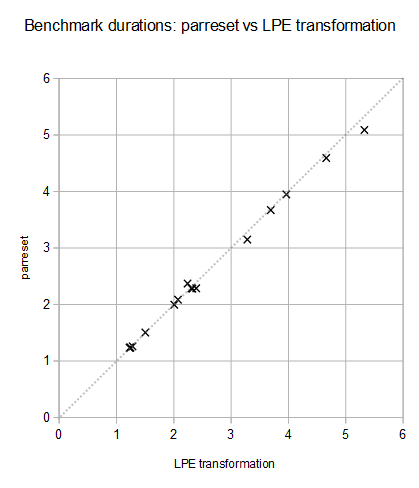
\includegraphics[width=0.7\linewidth]{charts/parreset-vs-lpe-only}
\caption{Benchmark results: parreset vs LPE transformation}
\label{parreset-vs-lpe-only:fig}
\end{center}
\end{figure}


